\documentclass[a4paper,11pt]{scrreprt}
\usepackage{amsmath}
\usepackage{amssymb}
\usepackage{tikz}
\usepackage{url}
\usepackage{lmodern}
\usepackage{microtype}

\newcommand*{\code}[1]{\texttt{#1}}
\newcommand*{\defi}[1]{\textbf{#1}}

\title{Technical supplement to the COVID19 report}
\author{Hugh Parsonage}

\providecommand{\crema}{\textsc{crema}}


\begin{document}

\addchap{Overview}
Our model, \crema, is a dynamic microsimulation model of Australia. 

\subsection{Static data}
The model runs on a static data table, each row a person in Australia, 
which identifies each person's

\begin{enumerate}
	\item state and SA2,
	\item age
	\item household
	\item school,
	\item labour force status,
\end{enumerate}

For performance reasons, data is cached before being passed to the dynamic model.
Obviously, the cache includes the static data. Other features of each person is 
also cached (or ``generated at cache time''). Cache time variables include:

\begin{description}
\item[\code{SupermarketTypical}] If an individual's SA2 contains zero supermarkets, 
a value of zero. 
For implementation convenience,%
	\footnote{By \defi{implementation convenience}, I mean that the choice was not made 
	on the basis of research, because it was necessary to do so and was not considered 
	sufficiently important to make more than an arbitrary decision. In this case,
	the choice of 8 was made to avoid stack overflow.}
If the individual's SA2 contains more than eight supermarket we 
exclude all but eight supermarkets. We then assign to each person a random integer
from 1 to \(N_S = {}\) the number of supermarkets in each SA2 to represent the 
`typical' supermarket a person visits.
\end{description}

For technical reasons, we shorten variables so that they are a sequence. 

\subsection{Assignment of individuals to workplaces}
While we are confident about the distribution of labour force status among
the population we assign in the static data, we do not know how large each 
worker's workplace is. To model this, for each destination zone we construct
a sequence of geometrically distributed random variables with parameters 
\(1/\beta = 1/15\). 

\begin{figure}[!htbp]
\caption{The geometric distribution with mean 15 over the range [0, 50]}\label{fig:geom-distr}
\makebox[\textwidth]{
	% Created by tikzDevice version 0.12.3 on 2020-05-31 18:14:11
% !TEX encoding = UTF-8 Unicode
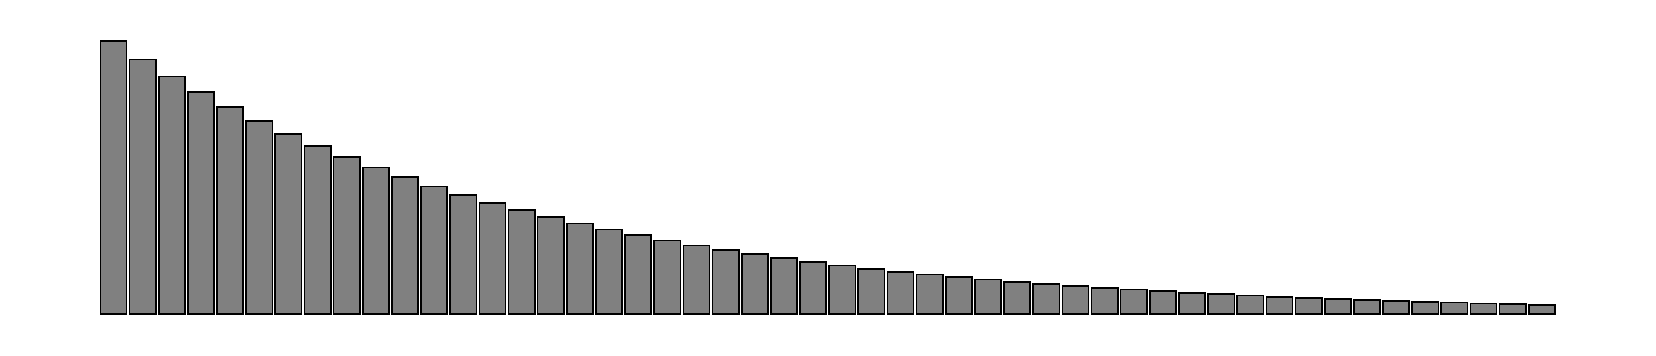
\begin{tikzpicture}[x=1pt,y=1pt]
\definecolor{fillColor}{RGB}{255,255,255}
\path[use as bounding box,fill=fillColor,fill opacity=0.00] (0,0) rectangle (578.16,108.41);
\begin{scope}
\path[clip] (  0.00,  0.00) rectangle (578.16,108.41);
\definecolor{drawColor}{RGB}{0,0,0}
\definecolor{fillColor}{RGB}{128,128,128}

\path[draw=drawColor,line width= 0.6pt,line cap=rect,fill=fillColor] ( 26.28,  4.93) rectangle ( 35.76,103.48);

\path[draw=drawColor,line width= 0.6pt,line cap=rect,fill=fillColor] ( 36.81,  4.93) rectangle ( 46.29, 96.91);

\path[draw=drawColor,line width= 0.6pt,line cap=rect,fill=fillColor] ( 47.35,  4.93) rectangle ( 56.83, 90.78);

\path[draw=drawColor,line width= 0.6pt,line cap=rect,fill=fillColor] ( 57.88,  4.93) rectangle ( 67.36, 85.05);

\path[draw=drawColor,line width= 0.6pt,line cap=rect,fill=fillColor] ( 68.41,  4.93) rectangle ( 77.89, 79.71);

\path[draw=drawColor,line width= 0.6pt,line cap=rect,fill=fillColor] ( 78.95,  4.93) rectangle ( 88.43, 74.73);

\path[draw=drawColor,line width= 0.6pt,line cap=rect,fill=fillColor] ( 89.48,  4.93) rectangle ( 98.96, 70.07);

\path[draw=drawColor,line width= 0.6pt,line cap=rect,fill=fillColor] (100.01,  4.93) rectangle (109.49, 65.73);

\path[draw=drawColor,line width= 0.6pt,line cap=rect,fill=fillColor] (110.54,  4.93) rectangle (120.02, 61.68);

\path[draw=drawColor,line width= 0.6pt,line cap=rect,fill=fillColor] (121.08,  4.93) rectangle (130.56, 57.89);

\path[draw=drawColor,line width= 0.6pt,line cap=rect,fill=fillColor] (131.61,  4.93) rectangle (141.09, 54.36);

\path[draw=drawColor,line width= 0.6pt,line cap=rect,fill=fillColor] (142.14,  4.93) rectangle (151.62, 51.07);

\path[draw=drawColor,line width= 0.6pt,line cap=rect,fill=fillColor] (152.68,  4.93) rectangle (162.16, 47.99);

\path[draw=drawColor,line width= 0.6pt,line cap=rect,fill=fillColor] (163.21,  4.93) rectangle (172.69, 45.12);

\path[draw=drawColor,line width= 0.6pt,line cap=rect,fill=fillColor] (173.74,  4.93) rectangle (183.22, 42.44);

\path[draw=drawColor,line width= 0.6pt,line cap=rect,fill=fillColor] (184.28,  4.93) rectangle (193.76, 39.94);

\path[draw=drawColor,line width= 0.6pt,line cap=rect,fill=fillColor] (194.81,  4.93) rectangle (204.29, 37.60);

\path[draw=drawColor,line width= 0.6pt,line cap=rect,fill=fillColor] (205.34,  4.93) rectangle (214.82, 35.43);

\path[draw=drawColor,line width= 0.6pt,line cap=rect,fill=fillColor] (215.88,  4.93) rectangle (225.35, 33.39);

\path[draw=drawColor,line width= 0.6pt,line cap=rect,fill=fillColor] (226.41,  4.93) rectangle (235.89, 31.50);

\path[draw=drawColor,line width= 0.6pt,line cap=rect,fill=fillColor] (236.94,  4.93) rectangle (246.42, 29.72);

\path[draw=drawColor,line width= 0.6pt,line cap=rect,fill=fillColor] (247.47,  4.93) rectangle (256.95, 28.07);

\path[draw=drawColor,line width= 0.6pt,line cap=rect,fill=fillColor] (258.01,  4.93) rectangle (267.49, 26.53);

\path[draw=drawColor,line width= 0.6pt,line cap=rect,fill=fillColor] (268.54,  4.93) rectangle (278.02, 25.09);

\path[draw=drawColor,line width= 0.6pt,line cap=rect,fill=fillColor] (279.07,  4.93) rectangle (288.55, 23.74);

\path[draw=drawColor,line width= 0.6pt,line cap=rect,fill=fillColor] (289.61,  4.93) rectangle (299.09, 22.49);

\path[draw=drawColor,line width= 0.6pt,line cap=rect,fill=fillColor] (300.14,  4.93) rectangle (309.62, 21.32);

\path[draw=drawColor,line width= 0.6pt,line cap=rect,fill=fillColor] (310.67,  4.93) rectangle (320.15, 20.23);

\path[draw=drawColor,line width= 0.6pt,line cap=rect,fill=fillColor] (321.21,  4.93) rectangle (330.69, 19.21);

\path[draw=drawColor,line width= 0.6pt,line cap=rect,fill=fillColor] (331.74,  4.93) rectangle (341.22, 18.25);

\path[draw=drawColor,line width= 0.6pt,line cap=rect,fill=fillColor] (342.27,  4.93) rectangle (351.75, 17.37);

\path[draw=drawColor,line width= 0.6pt,line cap=rect,fill=fillColor] (352.81,  4.93) rectangle (362.28, 16.54);

\path[draw=drawColor,line width= 0.6pt,line cap=rect,fill=fillColor] (363.34,  4.93) rectangle (372.82, 15.76);

\path[draw=drawColor,line width= 0.6pt,line cap=rect,fill=fillColor] (373.87,  4.93) rectangle (383.35, 15.04);

\path[draw=drawColor,line width= 0.6pt,line cap=rect,fill=fillColor] (384.40,  4.93) rectangle (393.88, 14.37);

\path[draw=drawColor,line width= 0.6pt,line cap=rect,fill=fillColor] (394.94,  4.93) rectangle (404.42, 13.74);

\path[draw=drawColor,line width= 0.6pt,line cap=rect,fill=fillColor] (405.47,  4.93) rectangle (414.95, 13.15);

\path[draw=drawColor,line width= 0.6pt,line cap=rect,fill=fillColor] (416.00,  4.93) rectangle (425.48, 12.60);

\path[draw=drawColor,line width= 0.6pt,line cap=rect,fill=fillColor] (426.54,  4.93) rectangle (436.02, 12.09);

\path[draw=drawColor,line width= 0.6pt,line cap=rect,fill=fillColor] (437.07,  4.93) rectangle (446.55, 11.61);

\path[draw=drawColor,line width= 0.6pt,line cap=rect,fill=fillColor] (447.60,  4.93) rectangle (457.08, 11.17);

\path[draw=drawColor,line width= 0.6pt,line cap=rect,fill=fillColor] (458.14,  4.93) rectangle (467.62, 10.75);

\path[draw=drawColor,line width= 0.6pt,line cap=rect,fill=fillColor] (468.67,  4.93) rectangle (478.15, 10.36);

\path[draw=drawColor,line width= 0.6pt,line cap=rect,fill=fillColor] (479.20,  4.93) rectangle (488.68, 10.00);

\path[draw=drawColor,line width= 0.6pt,line cap=rect,fill=fillColor] (489.73,  4.93) rectangle (499.21,  9.66);

\path[draw=drawColor,line width= 0.6pt,line cap=rect,fill=fillColor] (500.27,  4.93) rectangle (509.75,  9.35);

\path[draw=drawColor,line width= 0.6pt,line cap=rect,fill=fillColor] (510.80,  4.93) rectangle (520.28,  9.05);

\path[draw=drawColor,line width= 0.6pt,line cap=rect,fill=fillColor] (521.33,  4.93) rectangle (530.81,  8.78);

\path[draw=drawColor,line width= 0.6pt,line cap=rect,fill=fillColor] (531.87,  4.93) rectangle (541.35,  8.52);

\path[draw=drawColor,line width= 0.6pt,line cap=rect,fill=fillColor] (542.40,  4.93) rectangle (551.88,  8.28);
\end{scope}
\end{tikzpicture}

}
\end{figure}

The number of random variables to generate is determined algorithmically: if the next random variable
would overflow into the next DZN, we fill the rest of the sequences with 2, which has the useful 
side-effect of inflating the number of partnerships to a number consistent with observation.
With this sequence we obtain, for each working person, a group of workers associated with each person 
and the size of their workplace.

Assignment of workplace information completes the data generated at cache time. All other personal
features are constructed anew at runtime. 

\subsection{Assignment of candidate incubation and illness }

Our next step is to construct vectors to reflect user-supplied epidemiological parameters.
We construct for each person the duration of their incubation period and illness should they
be infected when the model starts. Although it would seem wasteful to generate these values
for every person, even if only a fraction of a percent of the rows are likely to be used, it 
so happens that this is more efficient than constructing them `just-in-time', mostly because
the model can perform large parts of its operation across the population in parallel, during 
which time the generation of random numbers is more difficult to coordinate.

The generation of the Poisson and log-normal distributions are done in the normal way using
 standard functions from the \code{stats} package.  For efficiency, we construct a small vector
 then use \code{rep\_len} to replicate it along the height of the data table. For example, if
 a Poisson distribution with parameter \(\lambda = 5\) is requested, we construct the vector

\[\text{\code{rep\_len(rpois(131059, 5), nrow(aus))}} \]

 For the Cauchy distribution, we implement our own version to allow for parallelized random
 number generation with an R seed. The Cauchy distribution is characterized by infrequent 
 extreme values so taking a small sample and repeating it was not adequate for this task.
 Since the Cauchy distribution has support over negative values,
 we use the absolute value.

\subsection{Reconstructing patient histories from the starting point}
The model accepts a starting date as an input, as an alternative to supplying the 
number and distribution of active and inactive cases in the population.
 To determine the number of active and inactive cases from a given starting date,
 we use a time series of each state's cumulative cases, together with assumptions
 about the source of each infection, and the epidemiological parameters that govern
 the duration of each persons' illness.%
 	\footnote{The time series data is from \url{https://github.com/pappubahry/AU_COVID19}, who
 	compiled the data from the state and territory health departments.}
 While some states
 	report recoveries and sources of infections, this information is not reported consistently
 	 (if at all) throughout the period.
Hence we are only able to \emph{estimate} the number of active cases at a point in time,
even if we take the data at face value. We assume that the cumulative number of cases
by date is correct, and we use the day-on-day difference of this number to reckon the
number of new cases. To each new case we assign a random member of the state's population and,
using the incubation and illness vectors allocated previously, determine the dates on which
the case was active.

Since a large number of new cases were from overseas arrivals, and since such individuals are more
likely to be quarantined from the population, we also need to estimate how many of the 
above cases would be in quarantine (and thus excluded from the model). We use the NSW and 
Victorian time series of infection sources to impute an overall percentage of new cases
on a given date that would be isolated and apply this percentage to all new cases to 
determine the number of new cases that exist in the wider community. On certain dates, 
in certain states,
the number of cases reported to have an overseas origin appears to exceed the \emph{total}
number of cases. In addition, the number of overseas cases is higher for earlier dates and 
becomes a less common source of infection after March. To moderate these effects, we subtract
the corresponding numbers of recovered patients in NSW and Victoria from both the number of 
overseas infections and the number of infections overall. We then take the average of the 
two percentages as the overall percentage of quarantined new infections on a particular date.
The number of deaths at the starting point is determined by the time series of deaths by state.

Otherwise, if the \code{InitialStatus} input is set, it is used to construct the initial status itself.

\section{PRNG}

Like most models of this nature, random number generation is both a core element and
a performance bottleneck.  We use a pseudo-random
number generator devised by Lehmer:\footnote{\url{https://lemire.me/blog/2019/03/19/the-fastest-conventional-random-number-generator-that-can-pass-big-crush/}}

\[x \mapsto \frac{(x \times 15750249268501108736)}{2^{64}}\]

The simplicity in the formulation makes seeding and parallelism relatively straightforward. We
provide a state space of 20 128-bit integers and simply cap the number of threads at 20 whenever
the PRNG is used. For uniformly distributed booleans of a fixed probability distribution
(as when applying transmission 
probabilities), we unpack the random number into \code{unsigned char} values as required. 
This array is seeded before each day, using R's PRNG's state, \code{.Random.seed} via 
the \code{dqrng} package.

\section{Infection model}

At the start of each day, various properties of the current state of the population is recorded, 
depending on the return type selected. In all cases, the number of active cases is recorded. 
If the number of active cases reaches zero, or the number of days to simulate is reached, the model
 terminates and these daily summaries returned.

Each person has a \textbf{Status} which is a 32-bit signed integer indicating whether or not
they are infected or have been infected, whether or not they are in isolation, and whether they are 
in intensive care. A status of zero indicates the person is susceptible to infection (but not
in isolation). Negative values indicate the person had been infected previously.


If an age-based lockdown is selected, the status of  all individuals of the ages requested have their
status flagged as isolated.

All infected individuals are then moved either from an incubation period to one of 
`symptomatic' or `critical', or from one of those status to `healed' or `killed', based
on the precomputed prognosis. 

Next, the person-to-person infection model runs, determined by the policy inputs and
the epidemiological inputs. Each person can be infected at a supermarket, a `place', 
a workplace, a school, at home, at a major event, or via a visit to another SA2. Each day
the order of these infectors is randomized, except that household infection always
occurs last. Following the modelling of household infection, contact tracing is performed,
if requested, and isolation applies for the next day.

\subsection{Supermarket infections}

Supermarkets are used to model basic interactions among people in the same suburb. 

Each person attends a supermarket 















\end{document}




